\documentclass[1p]{elsarticle_modified}
%\bibliographystyle{elsarticle-num}

%\usepackage[colorlinks]{hyperref}
%\usepackage{abbrmath_seonhwa} %\Abb, \Ascr, \Acal ,\Abf, \Afrak
\usepackage{amsfonts}
\usepackage{amssymb}
\usepackage{amsmath}
\usepackage{amsthm}
\usepackage{scalefnt}
\usepackage{amsbsy}
\usepackage{kotex}
\usepackage{caption}
\usepackage{subfig}
\usepackage{color}
\usepackage{graphicx}
\usepackage{xcolor} %% white, black, red, green, blue, cyan, magenta, yellow
\usepackage{float}
\usepackage{setspace}
\usepackage{hyperref}

\usepackage{tikz}
\usetikzlibrary{arrows}

\usepackage{multirow}
\usepackage{array} % fixed length table
\usepackage{hhline}

%%%%%%%%%%%%%%%%%%%%%
\makeatletter
\renewcommand*\env@matrix[1][\arraystretch]{%
	\edef\arraystretch{#1}%
	\hskip -\arraycolsep
	\let\@ifnextchar\new@ifnextchar
	\array{*\c@MaxMatrixCols c}}
\makeatother %https://tex.stackexchange.com/questions/14071/how-can-i-increase-the-line-spacing-in-a-matrix
%%%%%%%%%%%%%%%

\usepackage[normalem]{ulem}

\newcommand{\msout}[1]{\ifmmode\text{\sout{\ensuremath{#1}}}\else\sout{#1}\fi}
%SOURCE: \msout is \stkout macro in https://tex.stackexchange.com/questions/20609/strikeout-in-math-mode

\newcommand{\cancel}[1]{
	\ifmmode
	{\color{red}\msout{#1}}
	\else
	{\color{red}\sout{#1}}
	\fi
}

\newcommand{\add}[1]{
	{\color{blue}\uwave{#1}}
}

\newcommand{\replace}[2]{
	\ifmmode
	{\color{red}\msout{#1}}{\color{blue}\uwave{#2}}
	\else
	{\color{red}\sout{#1}}{\color{blue}\uwave{#2}}
	\fi
}

\newcommand{\Sol}{\mathcal{S}} %segment
\newcommand{\D}{D} %diagram
\newcommand{\A}{\mathcal{A}} %arc


%%%%%%%%%%%%%%%%%%%%%%%%%%%%%5 test

\def\sl{\operatorname{\textup{SL}}(2,\Cbb)}
\def\psl{\operatorname{\textup{PSL}}(2,\Cbb)}
\def\quan{\mkern 1mu \triangleright \mkern 1mu}

\theoremstyle{definition}
\newtheorem{thm}{Theorem}[section]
\newtheorem{prop}[thm]{Proposition}
\newtheorem{lem}[thm]{Lemma}
\newtheorem{ques}[thm]{Question}
\newtheorem{cor}[thm]{Corollary}
\newtheorem{defn}[thm]{Definition}
\newtheorem{exam}[thm]{Example}
\newtheorem{rmk}[thm]{Remark}
\newtheorem{alg}[thm]{Algorithm}

\newcommand{\I}{\sqrt{-1}}
\begin{document}

%\begin{frontmatter}
%
%\title{Boundary parabolic representations of knots up to 8 crossings}
%
%%% Group authors per affiliation:
%\author{Yunhi Cho} 
%\address{Department of Mathematics, University of Seoul, Seoul, Korea}
%\ead{yhcho@uos.ac.kr}
%
%
%\author{Seonhwa Kim} %\fnref{s_kim}}
%\address{Center for Geometry and Physics, Institute for Basic Science, Pohang, 37673, Korea}
%\ead{ryeona17@ibs.re.kr}
%
%\author{Hyuk Kim}
%\address{Department of Mathematical Sciences, Seoul National University, Seoul 08826, Korea}
%\ead{hyukkim@snu.ac.kr}
%
%\author{Seokbeom Yoon}
%\address{Department of Mathematical Sciences, Seoul National University, Seoul, 08826,  Korea}
%\ead{sbyoon15@snu.ac.kr}
%
%\begin{abstract}
%We find all boundary parabolic representation of knots up to 8 crossings.
%
%\end{abstract}
%\begin{keyword}
%    \MSC[2010] 57M25 
%\end{keyword}
%
%\end{frontmatter}

%\linenumbers
%\tableofcontents
%
\newcommand\colored[1]{\textcolor{white}{\rule[-0.35ex]{0.8em}{1.4ex}}\kern-0.8em\color{red} #1}%
%\newcommand\colored[1]{\textcolor{white}{ #1}\kern-2.17ex	\textcolor{white}{ #1}\kern-1.81ex	\textcolor{white}{ #1}\kern-2.15ex\color{red}#1	}

{\Large $\underline{12a_{1241}~(K12a_{1241})}$}

\setlength{\tabcolsep}{10pt}
\renewcommand{\arraystretch}{1.6}
\vspace{1cm}\begin{tabular}{m{100pt}>{\centering\arraybackslash}m{274pt}}
\multirow{5}{120pt}{
	\centering
	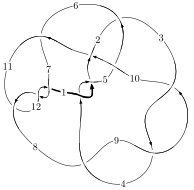
\includegraphics[width=112pt]{../../../GIT/diagram.site/Diagrams/png/2042_12a_1241.png}\\
\ \ \ A knot diagram\footnotemark}&
\allowdisplaybreaks
\textbf{Linearized knot diagam} \\
\cline{2-2}
 &
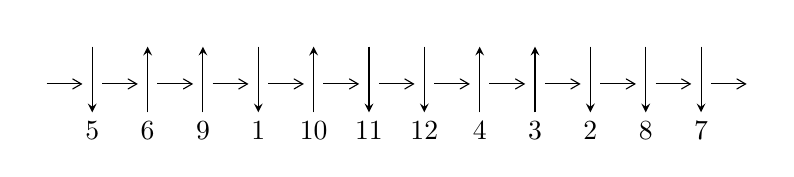
\begin{tikzpicture}[x=20pt, y=17pt]
	% nodes
	\node (C0) at (0, 0) {};
	\node (C1) at (1, 0) {};
	\node (C1U) at (1, +1) {};
	\node (C1D) at (1, -1) {5};

	\node (C2) at (2, 0) {};
	\node (C2U) at (2, +1) {};
	\node (C2D) at (2, -1) {6};

	\node (C3) at (3, 0) {};
	\node (C3U) at (3, +1) {};
	\node (C3D) at (3, -1) {9};

	\node (C4) at (4, 0) {};
	\node (C4U) at (4, +1) {};
	\node (C4D) at (4, -1) {1};

	\node (C5) at (5, 0) {};
	\node (C5U) at (5, +1) {};
	\node (C5D) at (5, -1) {10};

	\node (C6) at (6, 0) {};
	\node (C6U) at (6, +1) {};
	\node (C6D) at (6, -1) {11};

	\node (C7) at (7, 0) {};
	\node (C7U) at (7, +1) {};
	\node (C7D) at (7, -1) {12};

	\node (C8) at (8, 0) {};
	\node (C8U) at (8, +1) {};
	\node (C8D) at (8, -1) {4};

	\node (C9) at (9, 0) {};
	\node (C9U) at (9, +1) {};
	\node (C9D) at (9, -1) {3};

	\node (C10) at (10, 0) {};
	\node (C10U) at (10, +1) {};
	\node (C10D) at (10, -1) {2};

	\node (C11) at (11, 0) {};
	\node (C11U) at (11, +1) {};
	\node (C11D) at (11, -1) {8};

	\node (C12) at (12, 0) {};
	\node (C12U) at (12, +1) {};
	\node (C12D) at (12, -1) {7};
	\node (C13) at (13, 0) {};

	% arrows
	\draw[->,>={angle 60}]
	(C0) edge (C1) (C1) edge (C2) (C2) edge (C3) (C3) edge (C4) (C4) edge (C5) (C5) edge (C6) (C6) edge (C7) (C7) edge (C8) (C8) edge (C9) (C9) edge (C10) (C10) edge (C11) (C11) edge (C12) (C12) edge (C13) ;	\draw[->,>=stealth]
	(C1U) edge (C1D) (C2D) edge (C2U) (C3D) edge (C3U) (C4U) edge (C4D) (C5D) edge (C5U) (C6U) edge (C6D) (C7U) edge (C7D) (C8D) edge (C8U) (C9D) edge (C9U) (C10U) edge (C10D) (C11U) edge (C11D) (C12U) edge (C12D) ;
	\end{tikzpicture} \\
\hhline{~~} \\& 
\textbf{Solving Sequence} \\ \cline{2-2} 
 &
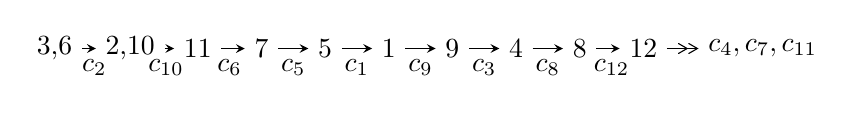
\begin{tikzpicture}[x=23pt, y=7pt]
	% node
	\node (A0) at (-1/8, 0) {3,6};
	\node (A1) at (17/16, 0) {2,10};
	\node (A2) at (17/8, 0) {11};
	\node (A3) at (25/8, 0) {7};
	\node (A4) at (33/8, 0) {5};
	\node (A5) at (41/8, 0) {1};
	\node (A6) at (49/8, 0) {9};
	\node (A7) at (57/8, 0) {4};
	\node (A8) at (65/8, 0) {8};
	\node (A9) at (73/8, 0) {12};
	\node (C1) at (1/2, -1) {$c_{2}$};
	\node (C2) at (13/8, -1) {$c_{10}$};
	\node (C3) at (21/8, -1) {$c_{6}$};
	\node (C4) at (29/8, -1) {$c_{5}$};
	\node (C5) at (37/8, -1) {$c_{1}$};
	\node (C6) at (45/8, -1) {$c_{9}$};
	\node (C7) at (53/8, -1) {$c_{3}$};
	\node (C8) at (61/8, -1) {$c_{8}$};
	\node (C9) at (69/8, -1) {$c_{12}$};
	\node (A10) at (11, 0) {$c_{4},c_{7},c_{11}$};

	% edge
	\draw[->,>=stealth]	
	(A0) edge (A1) (A1) edge (A2) (A2) edge (A3) (A3) edge (A4) (A4) edge (A5) (A5) edge (A6) (A6) edge (A7) (A7) edge (A8) (A8) edge (A9) ;
	\draw[->>,>={angle 60}]	
	(A9) edge (A10);
\end{tikzpicture} \\ 

\end{tabular} \\

\footnotetext{
The image of knot diagram is generated by the software ``\textbf{Draw programme}" developed by Andrew Bartholomew(\url{http://www.layer8.co.uk/maths/draw/index.htm\#Running-draw}), where we modified some parts for our purpose(\url{https://github.com/CATsTAILs/LinksPainter}).
}\phantom \\ \newline 
\centering \textbf{Ideals for irreducible components\footnotemark of $X_{\text{par}}$} 
 
\begin{align*}
I^u_{1}&=\langle 
5.62020\times10^{506} u^{97}+3.30268\times10^{507} u^{96}+\cdots+1.26259\times10^{508} b-1.88289\times10^{510},\\
\phantom{I^u_{1}}&\phantom{= \langle  }1.51364\times10^{508} u^{97}+4.93052\times10^{508} u^{96}+\cdots+3.04411\times10^{511} a-6.63987\times10^{513},\\
\phantom{I^u_{1}}&\phantom{= \langle  }u^{98}+7 u^{97}+\cdots+6163 u+2411\rangle \\
I^u_{2}&=\langle 
-35958023 u^{20}-5871878 u^{19}+\cdots+82788619 b+51534009,\\
\phantom{I^u_{2}}&\phantom{= \langle  }28948786 u^{20}-9908114 u^{19}+\cdots+82788619 a+47650307,\;u^{21}+3 u^{19}+\cdots+4 u^3-1\rangle \\
\\
\end{align*}
\raggedright * 2 irreducible components of $\dim_{\mathbb{C}}=0$, with total 119 representations.\\
\footnotetext{All coefficients of polynomials are rational numbers. But the coefficients are sometimes approximated in decimal forms when there is not enough margin.}
\newpage
\renewcommand{\arraystretch}{1}
\centering \section*{I. $I^u_{1}= \langle 5.62\times10^{506} u^{97}+3.30\times10^{507} u^{96}+\cdots+1.26\times10^{508} b-1.88\times10^{510},\;1.51\times10^{508} u^{97}+4.93\times10^{508} u^{96}+\cdots+3.04\times10^{511} a-6.64\times10^{513},\;u^{98}+7 u^{97}+\cdots+6163 u+2411 \rangle$}
\flushleft \textbf{(i) Arc colorings}\\
\begin{tabular}{m{7pt} m{180pt} m{7pt} m{180pt} }
\flushright $a_{3}=$&$\begin{pmatrix}1\\0\end{pmatrix}$ \\
\flushright $a_{6}=$&$\begin{pmatrix}0\\u\end{pmatrix}$ \\
\flushright $a_{2}=$&$\begin{pmatrix}1\\u^2\end{pmatrix}$ \\
\flushright $a_{10}=$&$\begin{pmatrix}-0.000497238 u^{97}-0.00161969 u^{96}+\cdots+444.575 u+218.122\\-0.0445132 u^{97}-0.261579 u^{96}+\cdots+164.459 u+149.129\end{pmatrix}$ \\
\flushright $a_{11}=$&$\begin{pmatrix}0.0435860 u^{97}+0.269441 u^{96}+\cdots+269.846 u+64.5064\\-0.0606907 u^{97}-0.356223 u^{96}+\cdots+289.418 u+239.593\end{pmatrix}$ \\
\flushright $a_{7}=$&$\begin{pmatrix}0.230430 u^{97}+1.78272 u^{96}+\cdots+3320.78 u+1062.60\\-0.0866751 u^{97}-0.662088 u^{96}+\cdots-1338.01 u-353.286\end{pmatrix}$ \\
\flushright $a_{5}=$&$\begin{pmatrix}0.299926 u^{97}+2.27131 u^{96}+\cdots+3812.28 u+1215.95\\-0.144750 u^{97}-1.03754 u^{96}+\cdots-1552.10 u-316.827\end{pmatrix}$ \\
\flushright $a_{1}=$&$\begin{pmatrix}-0.142659 u^{97}-1.24303 u^{96}+\cdots-3628.12 u-1358.82\\0.0981813 u^{97}+0.780441 u^{96}+\cdots+1918.65 u+630.422\end{pmatrix}$ \\
\flushright $a_{9}=$&$\begin{pmatrix}0.0440160 u^{97}+0.259960 u^{96}+\cdots+280.116 u+68.9932\\-0.0445132 u^{97}-0.261579 u^{96}+\cdots+164.459 u+149.129\end{pmatrix}$ \\
\flushright $a_{4}=$&$\begin{pmatrix}0.163505 u^{97}+0.986985 u^{96}+\cdots-1062.50 u-885.931\\-0.0320956 u^{97}-0.211873 u^{96}+\cdots+194.491 u+143.704\end{pmatrix}$ \\
\flushright $a_{8}=$&$\begin{pmatrix}-0.0452535 u^{97}-0.318641 u^{96}+\cdots-510.276 u-346.848\\0.0816803 u^{97}+0.517141 u^{96}+\cdots+179.363 u-83.0401\end{pmatrix}$ \\
\flushright $a_{12}=$&$\begin{pmatrix}0.0571524 u^{97}+0.334182 u^{96}+\cdots+137.694 u-213.754\\-0.0435898 u^{97}-0.259607 u^{96}+\cdots+177.399 u+261.550\end{pmatrix}$\\&\end{tabular}
\flushleft \textbf{(ii) Obstruction class $= -1$}\\~\\
\flushleft \textbf{(iii) Cusp Shapes $= -0.161576 u^{97}-1.15515 u^{96}+\cdots-1184.37 u-255.285$}\\~\\
\newpage\renewcommand{\arraystretch}{1}
\flushleft \textbf{(iv) u-Polynomials at the component}\newline \\
\begin{tabular}{m{50pt}|m{274pt}}
Crossings & \hspace{64pt}u-Polynomials at each crossing \\
\hline $$\begin{aligned}c_{1},c_{4}\end{aligned}$$&$\begin{aligned}
&u^{98}-2 u^{97}+\cdots+454 u+52
\end{aligned}$\\
\hline $$\begin{aligned}c_{2}\end{aligned}$$&$\begin{aligned}
&u^{98}-7 u^{97}+\cdots-6163 u+2411
\end{aligned}$\\
\hline $$\begin{aligned}c_{3},c_{8},c_{9}\end{aligned}$$&$\begin{aligned}
&u^{98}+u^{97}+\cdots-625 u+77
\end{aligned}$\\
\hline $$\begin{aligned}c_{5}\end{aligned}$$&$\begin{aligned}
&u^{98}+3 u^{97}+\cdots+18901 u+4059
\end{aligned}$\\
\hline $$\begin{aligned}c_{6}\end{aligned}$$&$\begin{aligned}
&u^{98}-30 u^{96}+\cdots+455 u+97
\end{aligned}$\\
\hline $$\begin{aligned}c_{7},c_{11},c_{12}\end{aligned}$$&$\begin{aligned}
&u^{98}+42 u^{96}+\cdots+17 u+1
\end{aligned}$\\
\hline $$\begin{aligned}c_{10}\end{aligned}$$&$\begin{aligned}
&u^{98}+5 u^{97}+\cdots+7783 u+1015
\end{aligned}$\\
\hline
\end{tabular}\\~\\
\newpage\renewcommand{\arraystretch}{1}
\flushleft \textbf{(v) Riley Polynomials at the component}\newline \\
\begin{tabular}{m{50pt}|m{274pt}}
Crossings & \hspace{64pt}Riley Polynomials at each crossing \\
\hline $$\begin{aligned}c_{1},c_{4}\end{aligned}$$&$\begin{aligned}
&y^{98}-86 y^{97}+\cdots+334372 y+2704
\end{aligned}$\\
\hline $$\begin{aligned}c_{2}\end{aligned}$$&$\begin{aligned}
&y^{98}+29 y^{97}+\cdots+216614209 y+5812921
\end{aligned}$\\
\hline $$\begin{aligned}c_{3},c_{8},c_{9}\end{aligned}$$&$\begin{aligned}
&y^{98}+107 y^{97}+\cdots+162543 y+5929
\end{aligned}$\\
\hline $$\begin{aligned}c_{5}\end{aligned}$$&$\begin{aligned}
&y^{98}+33 y^{97}+\cdots+550117295 y+16475481
\end{aligned}$\\
\hline $$\begin{aligned}c_{6}\end{aligned}$$&$\begin{aligned}
&y^{98}-60 y^{97}+\cdots+4415607 y+9409
\end{aligned}$\\
\hline $$\begin{aligned}c_{7},c_{11},c_{12}\end{aligned}$$&$\begin{aligned}
&y^{98}+84 y^{97}+\cdots+511 y+1
\end{aligned}$\\
\hline $$\begin{aligned}c_{10}\end{aligned}$$&$\begin{aligned}
&y^{98}-23 y^{97}+\cdots-47629779 y+1030225
\end{aligned}$\\
\hline
\end{tabular}\\~\\
\newpage\flushleft \textbf{(vi) Complex Volumes and Cusp Shapes}
$$\begin{array}{c|c|c}  
\text{Solutions to }I^u_{1}& \I (\text{vol} + \sqrt{-1}CS) & \text{Cusp shape}\\
 \hline 
\begin{aligned}
u &= \phantom{-}0.253022 + 0.971744 I \\
a &= \phantom{-}1.228300 - 0.565343 I \\
b &= \phantom{-}0.22606 + 1.48582 I\end{aligned}
 & -4.47832 + 4.71335 I & \phantom{-0.000000 } 0 \\ \hline\begin{aligned}
u &= \phantom{-}0.253022 - 0.971744 I \\
a &= \phantom{-}1.228300 + 0.565343 I \\
b &= \phantom{-}0.22606 - 1.48582 I\end{aligned}
 & -4.47832 - 4.71335 I & \phantom{-0.000000 } 0 \\ \hline\begin{aligned}
u &= -0.361168 + 0.912422 I \\
a &= -0.938996 - 0.090557 I \\
b &= -1.102380 - 0.355055 I\end{aligned}
 & -1.31097 + 1.94718 I & \phantom{-0.000000 } 0 \\ \hline\begin{aligned}
u &= -0.361168 - 0.912422 I \\
a &= -0.938996 + 0.090557 I \\
b &= -1.102380 + 0.355055 I\end{aligned}
 & -1.31097 - 1.94718 I & \phantom{-0.000000 } 0 \\ \hline\begin{aligned}
u &= -0.953890 + 0.418609 I \\
a &= -0.897666 + 0.239337 I \\
b &= -0.676448 + 0.223462 I\end{aligned}
 & \phantom{-}6.31069 - 0.36260 I & \phantom{-0.000000 } 0 \\ \hline\begin{aligned}
u &= -0.953890 - 0.418609 I \\
a &= -0.897666 - 0.239337 I \\
b &= -0.676448 - 0.223462 I\end{aligned}
 & \phantom{-}6.31069 + 0.36260 I & \phantom{-0.000000 } 0 \\ \hline\begin{aligned}
u &= -0.086926 + 1.046640 I \\
a &= -0.855169 - 0.016414 I \\
b &= -0.41197 + 1.62733 I\end{aligned}
 & -7.82875 - 7.69575 I & \phantom{-0.000000 } 0 \\ \hline\begin{aligned}
u &= -0.086926 - 1.046640 I \\
a &= -0.855169 + 0.016414 I \\
b &= -0.41197 - 1.62733 I\end{aligned}
 & -7.82875 + 7.69575 I & \phantom{-0.000000 } 0 \\ \hline\begin{aligned}
u &= \phantom{-}0.732080 + 0.574872 I \\
a &= \phantom{-}1.35164 + 0.54134 I \\
b &= \phantom{-}0.527080 + 0.217054 I\end{aligned}
 & \phantom{-}4.60166 + 4.95582 I & \phantom{-0.000000 } 0 \\ \hline\begin{aligned}
u &= \phantom{-}0.732080 - 0.574872 I \\
a &= \phantom{-}1.35164 - 0.54134 I \\
b &= \phantom{-}0.527080 - 0.217054 I\end{aligned}
 & \phantom{-}4.60166 - 4.95582 I & \phantom{-0.000000 } 0\\
 \hline 
 \end{array}$$\newpage$$\begin{array}{c|c|c}  
\text{Solutions to }I^u_{1}& \I (\text{vol} + \sqrt{-1}CS) & \text{Cusp shape}\\
 \hline 
\begin{aligned}
u &= -0.151039 + 0.912026 I \\
a &= \phantom{-}0.965108 - 0.073747 I \\
b &= \phantom{-}0.34093 - 1.67994 I\end{aligned}
 & -12.49310 - 3.58757 I & \phantom{-0.000000 } 0 \\ \hline\begin{aligned}
u &= -0.151039 - 0.912026 I \\
a &= \phantom{-}0.965108 + 0.073747 I \\
b &= \phantom{-}0.34093 + 1.67994 I\end{aligned}
 & -12.49310 + 3.58757 I & \phantom{-0.000000 } 0 \\ \hline\begin{aligned}
u &= \phantom{-}0.719249 + 0.578215 I \\
a &= \phantom{-}0.510756 + 0.568805 I \\
b &= \phantom{-}0.319764 - 0.549263 I\end{aligned}
 & \phantom{-}3.90783 + 4.05242 I & \phantom{-0.000000 } 0 \\ \hline\begin{aligned}
u &= \phantom{-}0.719249 - 0.578215 I \\
a &= \phantom{-}0.510756 - 0.568805 I \\
b &= \phantom{-}0.319764 + 0.549263 I\end{aligned}
 & \phantom{-}3.90783 - 4.05242 I & \phantom{-0.000000 } 0 \\ \hline\begin{aligned}
u &= \phantom{-}0.011715 + 0.911513 I \\
a &= \phantom{-}0.751748 + 0.335932 I \\
b &= \phantom{-}0.598604 - 0.265419 I\end{aligned}
 & \phantom{-}1.37687 - 1.50928 I & \phantom{-0.000000 } 0 \\ \hline\begin{aligned}
u &= \phantom{-}0.011715 - 0.911513 I \\
a &= \phantom{-}0.751748 - 0.335932 I \\
b &= \phantom{-}0.598604 + 0.265419 I\end{aligned}
 & \phantom{-}1.37687 + 1.50928 I & \phantom{-0.000000 } 0 \\ \hline\begin{aligned}
u &= -0.411815 + 0.812519 I \\
a &= \phantom{-}1.030430 + 0.031946 I \\
b &= \phantom{-}1.076620 + 0.516415 I\end{aligned}
 & -5.12526 - 1.90924 I & \phantom{-0.000000 } 0 \\ \hline\begin{aligned}
u &= -0.411815 - 0.812519 I \\
a &= \phantom{-}1.030430 - 0.031946 I \\
b &= \phantom{-}1.076620 - 0.516415 I\end{aligned}
 & -5.12526 + 1.90924 I & \phantom{-0.000000 } 0 \\ \hline\begin{aligned}
u &= -0.555460 + 0.700572 I \\
a &= -2.65690 + 0.21983 I \\
b &= -0.02164 + 1.53493 I\end{aligned}
 & -9.53244 - 4.05758 I & \phantom{-0.000000 } 0 \\ \hline\begin{aligned}
u &= -0.555460 - 0.700572 I \\
a &= -2.65690 - 0.21983 I \\
b &= -0.02164 - 1.53493 I\end{aligned}
 & -9.53244 + 4.05758 I & \phantom{-0.000000 } 0\\
 \hline 
 \end{array}$$\newpage$$\begin{array}{c|c|c}  
\text{Solutions to }I^u_{1}& \I (\text{vol} + \sqrt{-1}CS) & \text{Cusp shape}\\
 \hline 
\begin{aligned}
u &= -0.477299 + 0.724656 I \\
a &= -1.101160 + 0.068783 I \\
b &= -1.080780 - 0.663592 I\end{aligned}
 & -1.04793 - 5.79172 I & \phantom{-0.000000 } 0 \\ \hline\begin{aligned}
u &= -0.477299 - 0.724656 I \\
a &= -1.101160 - 0.068783 I \\
b &= -1.080780 + 0.663592 I\end{aligned}
 & -1.04793 + 5.79172 I & \phantom{-0.000000 } 0 \\ \hline\begin{aligned}
u &= \phantom{-}0.234186 + 0.806850 I \\
a &= -1.68852 + 0.70590 I \\
b &= -0.096508 - 0.608610 I\end{aligned}
 & -2.46525 + 3.67993 I & \phantom{-0.000000 } 0 \\ \hline\begin{aligned}
u &= \phantom{-}0.234186 - 0.806850 I \\
a &= -1.68852 - 0.70590 I \\
b &= -0.096508 + 0.608610 I\end{aligned}
 & -2.46525 - 3.67993 I & \phantom{-0.000000 } 0 \\ \hline\begin{aligned}
u &= \phantom{-}0.293389 + 1.155010 I \\
a &= -1.051790 + 0.520303 I \\
b &= -0.091467 - 0.999276 I\end{aligned}
 & -2.63731 + 3.64297 I & \phantom{-0.000000 } 0 \\ \hline\begin{aligned}
u &= \phantom{-}0.293389 - 1.155010 I \\
a &= -1.051790 - 0.520303 I \\
b &= -0.091467 + 0.999276 I\end{aligned}
 & -2.63731 - 3.64297 I & \phantom{-0.000000 } 0 \\ \hline\begin{aligned}
u &= -0.511481 + 0.622118 I \\
a &= \phantom{-}0.941842 + 0.089696 I \\
b &= \phantom{-}0.476021 - 0.247877 I\end{aligned}
 & \phantom{-}0.762154 - 1.099890 I & \phantom{-0.000000 } 0 \\ \hline\begin{aligned}
u &= -0.511481 - 0.622118 I \\
a &= \phantom{-}0.941842 - 0.089696 I \\
b &= \phantom{-}0.476021 + 0.247877 I\end{aligned}
 & \phantom{-}0.762154 + 1.099890 I & \phantom{-0.000000 } 0 \\ \hline\begin{aligned}
u &= \phantom{-}0.140471 + 0.791468 I \\
a &= -1.43894 + 0.87695 I \\
b &= -0.10479 - 1.50633 I\end{aligned}
 & -7.69184 + 0.59503 I & \phantom{-0.000000 } 0 \\ \hline\begin{aligned}
u &= \phantom{-}0.140471 - 0.791468 I \\
a &= -1.43894 - 0.87695 I \\
b &= -0.10479 + 1.50633 I\end{aligned}
 & -7.69184 - 0.59503 I & \phantom{-0.000000 } 0\\
 \hline 
 \end{array}$$\newpage$$\begin{array}{c|c|c}  
\text{Solutions to }I^u_{1}& \I (\text{vol} + \sqrt{-1}CS) & \text{Cusp shape}\\
 \hline 
\begin{aligned}
u &= -0.968387 + 0.758823 I \\
a &= -0.452375 + 0.502174 I \\
b &= -0.07400 + 1.60154 I\end{aligned}
 & -9.10905 - 0.25018 I & \phantom{-0.000000 } 0 \\ \hline\begin{aligned}
u &= -0.968387 - 0.758823 I \\
a &= -0.452375 - 0.502174 I \\
b &= -0.07400 - 1.60154 I\end{aligned}
 & -9.10905 + 0.25018 I & \phantom{-0.000000 } 0 \\ \hline\begin{aligned}
u &= -0.582839 + 0.494454 I \\
a &= \phantom{-}0.59706 + 1.83322 I \\
b &= \phantom{-}0.513909 - 0.332393 I\end{aligned}
 & \phantom{-}0.10343 - 5.42157 I & \phantom{-0.000000 -}0. + 9.49655 I \\ \hline\begin{aligned}
u &= -0.582839 - 0.494454 I \\
a &= \phantom{-}0.59706 - 1.83322 I \\
b &= \phantom{-}0.513909 + 0.332393 I\end{aligned}
 & \phantom{-}0.10343 + 5.42157 I & \phantom{-0.000000 } 0. - 9.49655 I \\ \hline\begin{aligned}
u &= \phantom{-}0.642839 + 1.056130 I \\
a &= -1.109050 + 0.101431 I \\
b &= -0.664693 - 0.827070 I\end{aligned}
 & -3.13702 + 3.92759 I & \phantom{-0.000000 } 0 \\ \hline\begin{aligned}
u &= \phantom{-}0.642839 - 1.056130 I \\
a &= -1.109050 - 0.101431 I \\
b &= -0.664693 + 0.827070 I\end{aligned}
 & -3.13702 - 3.92759 I & \phantom{-0.000000 } 0 \\ \hline\begin{aligned}
u &= -0.181205 + 1.275240 I \\
a &= \phantom{-}0.589758 + 0.246208 I \\
b &= \phantom{-}0.183271 - 0.218860 I\end{aligned}
 & \phantom{-}1.51179 - 1.16300 I & \phantom{-0.000000 } 0 \\ \hline\begin{aligned}
u &= -0.181205 - 1.275240 I \\
a &= \phantom{-}0.589758 - 0.246208 I \\
b &= \phantom{-}0.183271 + 0.218860 I\end{aligned}
 & \phantom{-}1.51179 + 1.16300 I & \phantom{-0.000000 } 0 \\ \hline\begin{aligned}
u &= -0.240973 + 0.664061 I \\
a &= -1.207900 + 0.353763 I \\
b &= -0.23164 + 1.74547 I\end{aligned}
 & -9.48090 + 0.46429 I & -9.33722 - 0.88532 I \\ \hline\begin{aligned}
u &= -0.240973 - 0.664061 I \\
a &= -1.207900 - 0.353763 I \\
b &= -0.23164 - 1.74547 I\end{aligned}
 & -9.48090 - 0.46429 I & -9.33722 + 0.88532 I\\
 \hline 
 \end{array}$$\newpage$$\begin{array}{c|c|c}  
\text{Solutions to }I^u_{1}& \I (\text{vol} + \sqrt{-1}CS) & \text{Cusp shape}\\
 \hline 
\begin{aligned}
u &= \phantom{-}0.676028 + 1.106150 I \\
a &= \phantom{-}1.013210 - 0.107878 I \\
b &= \phantom{-}0.176915 + 1.347300 I\end{aligned}
 & -4.23006 + 3.45286 I & \phantom{-0.000000 } 0 \\ \hline\begin{aligned}
u &= \phantom{-}0.676028 - 1.106150 I \\
a &= \phantom{-}1.013210 + 0.107878 I \\
b &= \phantom{-}0.176915 - 1.347300 I\end{aligned}
 & -4.23006 - 3.45286 I & \phantom{-0.000000 } 0 \\ \hline\begin{aligned}
u &= \phantom{-}0.386745 + 0.579689 I \\
a &= -0.643360 - 0.550780 I \\
b &= -0.363776 + 0.467216 I\end{aligned}
 & -1.20735 + 1.03467 I & -4.78917 + 0. I\phantom{ +0.000000I} \\ \hline\begin{aligned}
u &= \phantom{-}0.386745 - 0.579689 I \\
a &= -0.643360 + 0.550780 I \\
b &= -0.363776 - 0.467216 I\end{aligned}
 & -1.20735 - 1.03467 I & -4.78917 + 0. I\phantom{ +0.000000I} \\ \hline\begin{aligned}
u &= \phantom{-}0.787509 + 1.051300 I \\
a &= \phantom{-}1.034020 + 0.011995 I \\
b &= \phantom{-}0.842973 + 0.733535 I\end{aligned}
 & -5.98704 + 8.16987 I & \phantom{-0.000000 } 0 \\ \hline\begin{aligned}
u &= \phantom{-}0.787509 - 1.051300 I \\
a &= \phantom{-}1.034020 - 0.011995 I \\
b &= \phantom{-}0.842973 - 0.733535 I\end{aligned}
 & -5.98704 - 8.16987 I & \phantom{-0.000000 } 0 \\ \hline\begin{aligned}
u &= -1.070030 + 0.777663 I \\
a &= \phantom{-}1.23144 - 0.75638 I \\
b &= \phantom{-}0.12152 - 1.46773 I\end{aligned}
 & -1.04050 - 7.00303 I & \phantom{-0.000000 } 0 \\ \hline\begin{aligned}
u &= -1.070030 - 0.777663 I \\
a &= \phantom{-}1.23144 + 0.75638 I \\
b &= \phantom{-}0.12152 + 1.46773 I\end{aligned}
 & -1.04050 + 7.00303 I & \phantom{-0.000000 } 0 \\ \hline\begin{aligned}
u &= \phantom{-}0.012621 + 0.673624 I \\
a &= \phantom{-}1.43960 - 1.30487 I \\
b &= \phantom{-}0.00251 + 1.51873 I\end{aligned}
 & -3.19203 - 3.60931 I & -3.60074 + 2.59640 I \\ \hline\begin{aligned}
u &= \phantom{-}0.012621 - 0.673624 I \\
a &= \phantom{-}1.43960 + 1.30487 I \\
b &= \phantom{-}0.00251 - 1.51873 I\end{aligned}
 & -3.19203 + 3.60931 I & -3.60074 - 2.59640 I\\
 \hline 
 \end{array}$$\newpage$$\begin{array}{c|c|c}  
\text{Solutions to }I^u_{1}& \I (\text{vol} + \sqrt{-1}CS) & \text{Cusp shape}\\
 \hline 
\begin{aligned}
u &= \phantom{-}0.669031 + 0.057218 I \\
a &= -0.882681 + 0.590887 I \\
b &= -0.355258 - 0.829069 I\end{aligned}
 & \phantom{-}4.45227 + 3.37263 I & \phantom{-}2.57498 - 4.45245 I \\ \hline\begin{aligned}
u &= \phantom{-}0.669031 - 0.057218 I \\
a &= -0.882681 - 0.590887 I \\
b &= -0.355258 + 0.829069 I\end{aligned}
 & \phantom{-}4.45227 - 3.37263 I & \phantom{-}2.57498 + 4.45245 I \\ \hline\begin{aligned}
u &= \phantom{-}0.070567 + 0.663650 I \\
a &= -0.965466 - 0.774419 I \\
b &= -0.401206 - 0.489636 I\end{aligned}
 & -1.70244 - 1.41603 I & -3.82463 - 4.35155 I \\ \hline\begin{aligned}
u &= \phantom{-}0.070567 - 0.663650 I \\
a &= -0.965466 + 0.774419 I \\
b &= -0.401206 + 0.489636 I\end{aligned}
 & -1.70244 + 1.41603 I & -3.82463 + 4.35155 I \\ \hline\begin{aligned}
u &= -0.274034 + 0.597207 I \\
a &= \phantom{-}0.58410 - 2.43839 I \\
b &= -0.306884 + 0.424273 I\end{aligned}
 & -4.73792 - 0.91594 I & -14.1775 + 7.1751 I \\ \hline\begin{aligned}
u &= -0.274034 - 0.597207 I \\
a &= \phantom{-}0.58410 + 2.43839 I \\
b &= -0.306884 - 0.424273 I\end{aligned}
 & -4.73792 + 0.91594 I & -14.1775 - 7.1751 I \\ \hline\begin{aligned}
u &= -0.782678 + 1.100260 I \\
a &= -0.674478 - 0.011090 I \\
b &= -0.426595 + 0.459532 I\end{aligned}
 & -1.08514 - 3.89925 I & \phantom{-0.000000 } 0 \\ \hline\begin{aligned}
u &= -0.782678 - 1.100260 I \\
a &= -0.674478 + 0.011090 I \\
b &= -0.426595 - 0.459532 I\end{aligned}
 & -1.08514 + 3.89925 I & \phantom{-0.000000 } 0 \\ \hline\begin{aligned}
u &= \phantom{-}0.872848 + 1.035340 I \\
a &= -0.992791 - 0.070139 I \\
b &= -0.933028 - 0.664235 I\end{aligned}
 & -1.25539 + 12.36790 I & \phantom{-0.000000 } 0 \\ \hline\begin{aligned}
u &= \phantom{-}0.872848 - 1.035340 I \\
a &= -0.992791 + 0.070139 I \\
b &= -0.933028 + 0.664235 I\end{aligned}
 & -1.25539 - 12.36790 I & \phantom{-0.000000 } 0\\
 \hline 
 \end{array}$$\newpage$$\begin{array}{c|c|c}  
\text{Solutions to }I^u_{1}& \I (\text{vol} + \sqrt{-1}CS) & \text{Cusp shape}\\
 \hline 
\begin{aligned}
u &= -0.179029 + 0.608657 I \\
a &= \phantom{-}3.54093 + 2.48800 I \\
b &= -0.06719 - 1.51489 I\end{aligned}
 & -11.28210 + 2.12682 I & -19.6517 - 0.8079 I \\ \hline\begin{aligned}
u &= -0.179029 - 0.608657 I \\
a &= \phantom{-}3.54093 - 2.48800 I \\
b &= -0.06719 + 1.51489 I\end{aligned}
 & -11.28210 - 2.12682 I & -19.6517 + 0.8079 I \\ \hline\begin{aligned}
u &= \phantom{-}0.089926 + 0.598124 I \\
a &= -0.84393 - 3.85606 I \\
b &= \phantom{-}0.14492 + 1.47331 I\end{aligned}
 & -5.84333 + 7.70252 I & -9.7981 - 11.2309 I \\ \hline\begin{aligned}
u &= \phantom{-}0.089926 - 0.598124 I \\
a &= -0.84393 + 3.85606 I \\
b &= \phantom{-}0.14492 - 1.47331 I\end{aligned}
 & -5.84333 - 7.70252 I & -9.7981 + 11.2309 I \\ \hline\begin{aligned}
u &= \phantom{-}1.271310 + 0.611048 I \\
a &= \phantom{-}0.001508 - 0.596122 I \\
b &= \phantom{-}0.359510 - 0.682661 I\end{aligned}
 & -1.01263 + 2.26697 I & \phantom{-0.000000 } 0 \\ \hline\begin{aligned}
u &= \phantom{-}1.271310 - 0.611048 I \\
a &= \phantom{-}0.001508 + 0.596122 I \\
b &= \phantom{-}0.359510 + 0.682661 I\end{aligned}
 & -1.01263 - 2.26697 I & \phantom{-0.000000 } 0 \\ \hline\begin{aligned}
u &= \phantom{-}1.090940 + 0.897595 I \\
a &= \phantom{-}0.118660 + 0.563108 I \\
b &= -0.330387 + 0.507102 I\end{aligned}
 & -4.98910 - 1.42208 I & \phantom{-0.000000 } 0 \\ \hline\begin{aligned}
u &= \phantom{-}1.090940 - 0.897595 I \\
a &= \phantom{-}0.118660 - 0.563108 I \\
b &= -0.330387 - 0.507102 I\end{aligned}
 & -4.98910 + 1.42208 I & \phantom{-0.000000 } 0 \\ \hline\begin{aligned}
u &= \phantom{-}1.15829 + 0.86848 I \\
a &= -0.794019 - 0.292135 I \\
b &= -0.259473 - 1.347090 I\end{aligned}
 & \phantom{-}1.36352 + 3.73435 I & \phantom{-0.000000 } 0 \\ \hline\begin{aligned}
u &= \phantom{-}1.15829 - 0.86848 I \\
a &= -0.794019 + 0.292135 I \\
b &= -0.259473 + 1.347090 I\end{aligned}
 & \phantom{-}1.36352 - 3.73435 I & \phantom{-0.000000 } 0\\
 \hline 
 \end{array}$$\newpage$$\begin{array}{c|c|c}  
\text{Solutions to }I^u_{1}& \I (\text{vol} + \sqrt{-1}CS) & \text{Cusp shape}\\
 \hline 
\begin{aligned}
u &= \phantom{-}0.509418 + 0.015335 I \\
a &= \phantom{-}0.685640 - 0.008444 I \\
b &= \phantom{-}0.110118 - 0.780072 I\end{aligned}
 & -0.661179 - 1.248990 I & -2.42504 + 5.87685 I \\ \hline\begin{aligned}
u &= \phantom{-}0.509418 - 0.015335 I \\
a &= \phantom{-}0.685640 + 0.008444 I \\
b &= \phantom{-}0.110118 + 0.780072 I\end{aligned}
 & -0.661179 + 1.248990 I & -2.42504 - 5.87685 I \\ \hline\begin{aligned}
u &= -1.02084 + 1.09369 I \\
a &= \phantom{-}0.652315 - 0.066750 I \\
b &= \phantom{-}0.521275 - 0.555138 I\end{aligned}
 & \phantom{-}3.74698 - 7.24813 I & \phantom{-0.000000 } 0 \\ \hline\begin{aligned}
u &= -1.02084 - 1.09369 I \\
a &= \phantom{-}0.652315 + 0.066750 I \\
b &= \phantom{-}0.521275 + 0.555138 I\end{aligned}
 & \phantom{-}3.74698 + 7.24813 I & \phantom{-0.000000 } 0 \\ \hline\begin{aligned}
u &= -0.88831 + 1.22196 I \\
a &= -1.164150 + 0.057315 I \\
b &= -0.20453 + 1.60891 I\end{aligned}
 & -11.15240 - 7.16359 I & \phantom{-0.000000 } 0 \\ \hline\begin{aligned}
u &= -0.88831 - 1.22196 I \\
a &= -1.164150 - 0.057315 I \\
b &= -0.20453 - 1.60891 I\end{aligned}
 & -11.15240 + 7.16359 I & \phantom{-0.000000 } 0 \\ \hline\begin{aligned}
u &= \phantom{-}0.98697 + 1.19362 I \\
a &= -0.193337 - 0.484475 I \\
b &= \phantom{-}0.352727 - 0.338516 I\end{aligned}
 & -1.04985 - 5.14578 I & \phantom{-0.000000 } 0 \\ \hline\begin{aligned}
u &= \phantom{-}0.98697 - 1.19362 I \\
a &= -0.193337 + 0.484475 I \\
b &= \phantom{-}0.352727 + 0.338516 I\end{aligned}
 & -1.04985 + 5.14578 I & \phantom{-0.000000 } 0 \\ \hline\begin{aligned}
u &= -0.76861 + 1.42402 I \\
a &= \phantom{-}0.487964 - 0.188076 I \\
b &= \phantom{-}0.13072 - 1.43122 I\end{aligned}
 & -2.88616 - 0.46954 I & \phantom{-0.000000 } 0 \\ \hline\begin{aligned}
u &= -0.76861 - 1.42402 I \\
a &= \phantom{-}0.487964 + 0.188076 I \\
b &= \phantom{-}0.13072 + 1.43122 I\end{aligned}
 & -2.88616 + 0.46954 I & \phantom{-0.000000 } 0\\
 \hline 
 \end{array}$$\newpage$$\begin{array}{c|c|c}  
\text{Solutions to }I^u_{1}& \I (\text{vol} + \sqrt{-1}CS) & \text{Cusp shape}\\
 \hline 
\begin{aligned}
u &= -0.96362 + 1.33021 I \\
a &= \phantom{-}1.024180 - 0.042463 I \\
b &= \phantom{-}0.26543 - 1.61976 I\end{aligned}
 & -13.7565 - 12.2933 I & \phantom{-0.000000 } 0 \\ \hline\begin{aligned}
u &= -0.96362 - 1.33021 I \\
a &= \phantom{-}1.024180 + 0.042463 I \\
b &= \phantom{-}0.26543 + 1.61976 I\end{aligned}
 & -13.7565 + 12.2933 I & \phantom{-0.000000 } 0 \\ \hline\begin{aligned}
u &= -0.211165 + 0.255277 I \\
a &= \phantom{-}2.83520 - 0.04950 I \\
b &= \phantom{-}0.551289 + 0.974623 I\end{aligned}
 & \phantom{-}2.41153 - 1.09819 I & -0.23981 + 2.82127 I \\ \hline\begin{aligned}
u &= -0.211165 - 0.255277 I \\
a &= \phantom{-}2.83520 + 0.04950 I \\
b &= \phantom{-}0.551289 - 0.974623 I\end{aligned}
 & \phantom{-}2.41153 + 1.09819 I & -0.23981 - 2.82127 I \\ \hline\begin{aligned}
u &= -1.03724 + 1.37921 I \\
a &= -0.946320 + 0.059889 I \\
b &= -0.31087 + 1.60890 I\end{aligned}
 & -8.6855 - 16.9635 I & \phantom{-0.000000 } 0 \\ \hline\begin{aligned}
u &= -1.03724 - 1.37921 I \\
a &= -0.946320 - 0.059889 I \\
b &= -0.31087 - 1.60890 I\end{aligned}
 & -8.6855 + 16.9635 I & \phantom{-0.000000 } 0 \\ \hline\begin{aligned}
u &= \phantom{-}0.79524 + 1.66544 I \\
a &= \phantom{-}0.652174 - 0.180397 I \\
b &= \phantom{-}0.04078 + 1.48538 I\end{aligned}
 & -4.40204 + 1.83496 I & \phantom{-0.000000 } 0 \\ \hline\begin{aligned}
u &= \phantom{-}0.79524 - 1.66544 I \\
a &= \phantom{-}0.652174 + 0.180397 I \\
b &= \phantom{-}0.04078 - 1.48538 I\end{aligned}
 & -4.40204 - 1.83496 I & \phantom{-0.000000 } 0 \\ \hline\begin{aligned}
u &= \phantom{-}1.00328 + 1.64054 I \\
a &= -0.628453 + 0.097365 I \\
b &= -0.11468 - 1.52643 I\end{aligned}
 & -7.75971 + 5.78094 I & \phantom{-0.000000 } 0 \\ \hline\begin{aligned}
u &= \phantom{-}1.00328 - 1.64054 I \\
a &= -0.628453 - 0.097365 I \\
b &= -0.11468 + 1.52643 I\end{aligned}
 & -7.75971 - 5.78094 I & \phantom{-0.000000 } 0\\
 \hline 
 \end{array}$$\newpage$$\begin{array}{c|c|c}  
\text{Solutions to }I^u_{1}& \I (\text{vol} + \sqrt{-1}CS) & \text{Cusp shape}\\
 \hline 
\begin{aligned}
u &= \phantom{-}1.16084 + 1.63108 I \\
a &= \phantom{-}0.598586 - 0.046585 I \\
b &= \phantom{-}0.16721 + 1.55416 I\end{aligned}
 & -3.32821 + 9.79518 I & \phantom{-0.000000 } 0 \\ \hline\begin{aligned}
u &= \phantom{-}1.16084 - 1.63108 I \\
a &= \phantom{-}0.598586 + 0.046585 I \\
b &= \phantom{-}0.16721 - 1.55416 I\end{aligned}
 & -3.32821 - 9.79518 I & \phantom{-0.000000 } 0 \\ \hline\begin{aligned}
u &= -1.89459 + 0.85168 I \\
a &= -0.175177 + 0.324024 I \\
b &= \phantom{-}0.05072 + 1.60993 I\end{aligned}
 & -8.94260 - 0.96211 I & \phantom{-0.000000 } 0 \\ \hline\begin{aligned}
u &= -1.89459 - 0.85168 I \\
a &= -0.175177 - 0.324024 I \\
b &= \phantom{-}0.05072 - 1.60993 I\end{aligned}
 & -8.94260 + 0.96211 I & \phantom{-0.000000 } 0 \\ \hline\begin{aligned}
u &= -1.77035 + 1.31272 I \\
a &= \phantom{-}0.239271 - 0.254991 I \\
b &= -0.08249 - 1.54381 I\end{aligned}
 & -11.94420 + 2.84627 I & \phantom{-0.000000 } 0 \\ \hline\begin{aligned}
u &= -1.77035 - 1.31272 I \\
a &= \phantom{-}0.239271 + 0.254991 I \\
b &= -0.08249 + 1.54381 I\end{aligned}
 & -11.94420 - 2.84627 I & \phantom{-0.000000 } 0 \\ \hline\begin{aligned}
u &= -1.72554 + 1.57449 I \\
a &= -0.254697 + 0.210266 I \\
b &= \phantom{-}0.11181 + 1.49815 I\end{aligned}
 & -7.26258 + 6.81165 I & \phantom{-0.000000 } 0 \\ \hline\begin{aligned}
u &= -1.72554 - 1.57449 I \\
a &= -0.254697 - 0.210266 I \\
b &= \phantom{-}0.11181 - 1.49815 I\end{aligned}
 & -7.26258 - 6.81165 I & \phantom{-0.000000 } 0\\
 \hline 
 \end{array}$$\newpage\newpage\renewcommand{\arraystretch}{1}
\centering \section*{II. $I^u_{2}= \langle -3.60\times10^{7} u^{20}-5.87\times10^{6} u^{19}+\cdots+8.28\times10^{7} b+5.15\times10^{7},\;2.89\times10^{7} u^{20}-9.91\times10^{6} u^{19}+\cdots+8.28\times10^{7} a+4.77\times10^{7},\;u^{21}+3 u^{19}+\cdots+4 u^3-1 \rangle$}
\flushleft \textbf{(i) Arc colorings}\\
\begin{tabular}{m{7pt} m{180pt} m{7pt} m{180pt} }
\flushright $a_{3}=$&$\begin{pmatrix}1\\0\end{pmatrix}$ \\
\flushright $a_{6}=$&$\begin{pmatrix}0\\u\end{pmatrix}$ \\
\flushright $a_{2}=$&$\begin{pmatrix}1\\u^2\end{pmatrix}$ \\
\flushright $a_{10}=$&$\begin{pmatrix}-0.349671 u^{20}+0.119680 u^{19}+\cdots-0.328416 u-0.575566\\0.434335 u^{20}+0.0709261 u^{19}+\cdots+0.538125 u-0.622477\end{pmatrix}$ \\
\flushright $a_{11}=$&$\begin{pmatrix}-0.425572 u^{20}-0.583010 u^{19}+\cdots-1.21621 u+0.166591\\0.840659 u^{20}+0.126118 u^{19}+\cdots+0.462224 u-1.32517\end{pmatrix}$ \\
\flushright $a_{7}=$&$\begin{pmatrix}-1.07577 u^{20}+0.626412 u^{19}+\cdots-0.347425 u-1.24751\\-0.0441834 u^{20}-0.193456 u^{19}+\cdots-0.554242 u+1.16960\end{pmatrix}$ \\
\flushright $a_{5}=$&$\begin{pmatrix}-0.221566 u^{20}+0.0501958 u^{19}+\cdots-1.68495 u+0.104535\\0.191143 u^{20}-0.380578 u^{19}+\cdots-0.0806184 u+0.859053\end{pmatrix}$ \\
\flushright $a_{1}=$&$\begin{pmatrix}-1.08062 u^{20}+0.859053 u^{19}+\cdots+1.12989 u+2.18515\\0.456808 u^{20}-0.473624 u^{19}+\cdots-1.88948 u-0.521525\end{pmatrix}$ \\
\flushright $a_{9}=$&$\begin{pmatrix}-0.784006 u^{20}+0.0487535 u^{19}+\cdots-0.866541 u+0.0469111\\0.434335 u^{20}+0.0709261 u^{19}+\cdots+0.538125 u-0.622477\end{pmatrix}$ \\
\flushright $a_{4}=$&$\begin{pmatrix}1.23963 u^{20}-0.0745222 u^{19}+\cdots+1.32610 u-0.271762\\-0.380578 u^{20}+0.265665 u^{19}+\cdots-0.140947 u+0.191143\end{pmatrix}$ \\
\flushright $a_{8}=$&$\begin{pmatrix}-0.684952 u^{20}+0.104535 u^{19}+\cdots-0.833063 u-0.210797\\-0.287508 u^{20}+0.447015 u^{19}+\cdots-0.272806 u+0.314656\end{pmatrix}$ \\
\flushright $a_{12}=$&$\begin{pmatrix}0.185703 u^{20}+0.0640186 u^{19}+\cdots-0.305374 u+0.258156\\0.0746521 u^{20}-0.109910 u^{19}+\cdots-0.342353 u-0.510214\end{pmatrix}$\\&\end{tabular}
\flushleft \textbf{(ii) Obstruction class $= 1$}\\~\\
\flushleft \textbf{(iii) Cusp Shapes $= -\frac{367253532}{82788619} u^{20}+\frac{83600533}{82788619} u^{19}+\cdots+\frac{462458306}{82788619} u-\frac{448782682}{82788619}$}\\~\\
\newpage\renewcommand{\arraystretch}{1}
\flushleft \textbf{(iv) u-Polynomials at the component}\newline \\
\begin{tabular}{m{50pt}|m{274pt}}
Crossings & \hspace{64pt}u-Polynomials at each crossing \\
\hline $$\begin{aligned}c_{1}\end{aligned}$$&$\begin{aligned}
&u^{21}+3 u^{20}+\cdots-3 u-1
\end{aligned}$\\
\hline $$\begin{aligned}c_{2}\end{aligned}$$&$\begin{aligned}
&u^{21}+3 u^{19}+\cdots+4 u^3-1
\end{aligned}$\\
\hline $$\begin{aligned}c_{3}\end{aligned}$$&$\begin{aligned}
&u^{21}+12 u^{19}+\cdots-3 u^2-1
\end{aligned}$\\
\hline $$\begin{aligned}c_{4}\end{aligned}$$&$\begin{aligned}
&u^{21}-3 u^{20}+\cdots-3 u+1
\end{aligned}$\\
\hline $$\begin{aligned}c_{5}\end{aligned}$$&$\begin{aligned}
&u^{21}+3 u^{19}+\cdots-3 u^2-1
\end{aligned}$\\
\hline $$\begin{aligned}c_{6}\end{aligned}$$&$\begin{aligned}
&u^{21}- u^{20}+\cdots+3 u^2-1
\end{aligned}$\\
\hline $$\begin{aligned}c_{7}\end{aligned}$$&$\begin{aligned}
&u^{21}+u^{20}+\cdots-2 u-1
\end{aligned}$\\
\hline $$\begin{aligned}c_{8},c_{9}\end{aligned}$$&$\begin{aligned}
&u^{21}+12 u^{19}+\cdots+3 u^2+1
\end{aligned}$\\
\hline $$\begin{aligned}c_{10}\end{aligned}$$&$\begin{aligned}
&u^{21}+2 u^{20}+\cdots-4 u^3+1
\end{aligned}$\\
\hline $$\begin{aligned}c_{11},c_{12}\end{aligned}$$&$\begin{aligned}
&u^{21}- u^{20}+\cdots-2 u+1
\end{aligned}$\\
\hline
\end{tabular}\\~\\
\newpage\renewcommand{\arraystretch}{1}
\flushleft \textbf{(v) Riley Polynomials at the component}\newline \\
\begin{tabular}{m{50pt}|m{274pt}}
Crossings & \hspace{64pt}Riley Polynomials at each crossing \\
\hline $$\begin{aligned}c_{1},c_{4}\end{aligned}$$&$\begin{aligned}
&y^{21}-21 y^{20}+\cdots+15 y-1
\end{aligned}$\\
\hline $$\begin{aligned}c_{2}\end{aligned}$$&$\begin{aligned}
&y^{21}+6 y^{20}+\cdots+4 y^2-1
\end{aligned}$\\
\hline $$\begin{aligned}c_{3},c_{8},c_{9}\end{aligned}$$&$\begin{aligned}
&y^{21}+24 y^{20}+\cdots-6 y-1
\end{aligned}$\\
\hline $$\begin{aligned}c_{5}\end{aligned}$$&$\begin{aligned}
&y^{21}+6 y^{20}+\cdots-6 y-1
\end{aligned}$\\
\hline $$\begin{aligned}c_{6}\end{aligned}$$&$\begin{aligned}
&y^{21}-7 y^{20}+\cdots+6 y-1
\end{aligned}$\\
\hline $$\begin{aligned}c_{7},c_{11},c_{12}\end{aligned}$$&$\begin{aligned}
&y^{21}+21 y^{20}+\cdots+6 y-1
\end{aligned}$\\
\hline $$\begin{aligned}c_{10}\end{aligned}$$&$\begin{aligned}
&y^{21}-6 y^{20}+\cdots-8 y^2-1
\end{aligned}$\\
\hline
\end{tabular}\\~\\
\newpage\flushleft \textbf{(vi) Complex Volumes and Cusp Shapes}
$$\begin{array}{c|c|c}  
\text{Solutions to }I^u_{2}& \I (\text{vol} + \sqrt{-1}CS) & \text{Cusp shape}\\
 \hline 
\begin{aligned}
u &= -0.407597 + 0.870717 I \\
a &= \phantom{-}0.680319 + 1.087480 I \\
b &= -0.18046 - 1.47117 I\end{aligned}
 & -5.51707 + 6.87921 I & -4.74851 - 2.86739 I \\ \hline\begin{aligned}
u &= -0.407597 - 0.870717 I \\
a &= \phantom{-}0.680319 - 1.087480 I \\
b &= -0.18046 + 1.47117 I\end{aligned}
 & -5.51707 - 6.87921 I & -4.74851 + 2.86739 I \\ \hline\begin{aligned}
u &= \phantom{-}0.094729 + 1.047450 I \\
a &= \phantom{-}0.561172 + 0.309540 I \\
b &= \phantom{-}0.480951 + 0.574674 I\end{aligned}
 & \phantom{-}1.329940 - 0.100531 I & -4.48837 - 1.47261 I \\ \hline\begin{aligned}
u &= \phantom{-}0.094729 - 1.047450 I \\
a &= \phantom{-}0.561172 - 0.309540 I \\
b &= \phantom{-}0.480951 - 0.574674 I\end{aligned}
 & \phantom{-}1.329940 + 0.100531 I & -4.48837 + 1.47261 I \\ \hline\begin{aligned}
u &= -0.580685 + 0.636837 I \\
a &= \phantom{-}0.947436 - 0.573177 I \\
b &= \phantom{-}0.195506 + 0.576897 I\end{aligned}
 & \phantom{-}3.38035 - 4.48387 I & -6.73945 + 6.02054 I \\ \hline\begin{aligned}
u &= -0.580685 - 0.636837 I \\
a &= \phantom{-}0.947436 + 0.573177 I \\
b &= \phantom{-}0.195506 - 0.576897 I\end{aligned}
 & \phantom{-}3.38035 + 4.48387 I & -6.73945 - 6.02054 I \\ \hline\begin{aligned}
u &= -0.673019 + 0.436808 I \\
a &= -1.65014 + 0.46045 I \\
b &= \phantom{-}0.09381 + 1.54272 I\end{aligned}
 & -10.54320 + 2.25396 I & -7.32485 - 1.89994 I \\ \hline\begin{aligned}
u &= -0.673019 - 0.436808 I \\
a &= -1.65014 - 0.46045 I \\
b &= \phantom{-}0.09381 - 1.54272 I\end{aligned}
 & -10.54320 - 2.25396 I & -7.32485 + 1.89994 I \\ \hline\begin{aligned}
u &= -0.172176 + 0.734347 I \\
a &= -1.150890 - 0.189980 I \\
b &= -0.327687 - 0.508652 I\end{aligned}
 & -1.96242 - 1.97147 I & -10.38839 + 7.19935 I \\ \hline\begin{aligned}
u &= -0.172176 - 0.734347 I \\
a &= -1.150890 + 0.189980 I \\
b &= -0.327687 + 0.508652 I\end{aligned}
 & -1.96242 + 1.97147 I & -10.38839 - 7.19935 I\\
 \hline 
 \end{array}$$\newpage$$\begin{array}{c|c|c}  
\text{Solutions to }I^u_{2}& \I (\text{vol} + \sqrt{-1}CS) & \text{Cusp shape}\\
 \hline 
\begin{aligned}
u &= \phantom{-}0.599944 + 0.405600 I \\
a &= \phantom{-}0.457584 - 0.789305 I \\
b &= -0.609912 - 0.214868 I\end{aligned}
 & -0.67685 - 4.01014 I & -3.90329 + 2.87470 I \\ \hline\begin{aligned}
u &= \phantom{-}0.599944 - 0.405600 I \\
a &= \phantom{-}0.457584 + 0.789305 I \\
b &= -0.609912 + 0.214868 I\end{aligned}
 & -0.67685 + 4.01014 I & -3.90329 - 2.87470 I \\ \hline\begin{aligned}
u &= -1.255920 + 0.286813 I \\
a &= \phantom{-}0.281896 - 0.479640 I \\
b &= -0.06568 - 1.67537 I\end{aligned}
 & -8.29699 - 1.29880 I & -1.40444 + 6.09499 I \\ \hline\begin{aligned}
u &= -1.255920 - 0.286813 I \\
a &= \phantom{-}0.281896 + 0.479640 I \\
b &= -0.06568 + 1.67537 I\end{aligned}
 & -8.29699 + 1.29880 I & -1.40444 - 6.09499 I \\ \hline\begin{aligned}
u &= \phantom{-}0.635071 + 1.167840 I \\
a &= -1.037320 + 0.119056 I \\
b &= -0.148982 - 1.265150 I\end{aligned}
 & -4.77902 + 3.72263 I & -12.7993 - 6.1964 I \\ \hline\begin{aligned}
u &= \phantom{-}0.635071 - 1.167840 I \\
a &= -1.037320 - 0.119056 I \\
b &= -0.148982 + 1.265150 I\end{aligned}
 & -4.77902 - 3.72263 I & -12.7993 + 6.1964 I \\ \hline\begin{aligned}
u &= \phantom{-}0.994776 + 0.915498 I \\
a &= \phantom{-}1.050060 + 0.469010 I \\
b &= \phantom{-}0.095962 + 1.246490 I\end{aligned}
 & \phantom{-}0.84337 + 5.57019 I & -2.71521 - 5.54678 I \\ \hline\begin{aligned}
u &= \phantom{-}0.994776 - 0.915498 I \\
a &= \phantom{-}1.050060 - 0.469010 I \\
b &= \phantom{-}0.095962 - 1.246490 I\end{aligned}
 & \phantom{-}0.84337 - 5.57019 I & -2.71521 + 5.54678 I \\ \hline\begin{aligned}
u &= \phantom{-}0.503863\phantom{ +0.000000I} \\
a &= -1.63350\phantom{ +0.000000I} \\
b &= \phantom{-}0.532145\phantom{ +0.000000I}\end{aligned}
 & -4.47496\phantom{ +0.000000I} & -8.88530\phantom{ +0.000000I} \\ \hline\begin{aligned}
u &= \phantom{-}0.51294 + 1.50845 I \\
a &= \phantom{-}0.676633 - 0.200309 I \\
b &= \phantom{-}0.200421 + 1.238650 I\end{aligned}
 & -1.14943 + 2.54928 I & -2.54552 - 2.42691 I\\
 \hline 
 \end{array}$$\newpage$$\begin{array}{c|c|c}  
\text{Solutions to }I^u_{2}& \I (\text{vol} + \sqrt{-1}CS) & \text{Cusp shape}\\
 \hline 
\begin{aligned}
u &= \phantom{-}0.51294 - 1.50845 I \\
a &= \phantom{-}0.676633 + 0.200309 I \\
b &= \phantom{-}0.200421 - 1.238650 I\end{aligned}
 & -1.14943 - 2.54928 I & -2.54552 + 2.42691 I\\
 \hline 
 \end{array}$$\newpage
\newpage\renewcommand{\arraystretch}{1}
\centering \section*{ III. u-Polynomials}
\begin{tabular}{m{50pt}|m{274pt}}
Crossings & \hspace{64pt}u-Polynomials at each crossing \\
\hline $$\begin{aligned}c_{1}\end{aligned}$$&$\begin{aligned}
&(u^{21}+3 u^{20}+\cdots-3 u-1)(u^{98}-2 u^{97}+\cdots+454 u+52)
\end{aligned}$\\
\hline $$\begin{aligned}c_{2}\end{aligned}$$&$\begin{aligned}
&(u^{21}+3 u^{19}+\cdots+4 u^3-1)(u^{98}-7 u^{97}+\cdots-6163 u+2411)
\end{aligned}$\\
\hline $$\begin{aligned}c_{3}\end{aligned}$$&$\begin{aligned}
&(u^{21}+12 u^{19}+\cdots-3 u^2-1)(u^{98}+u^{97}+\cdots-625 u+77)
\end{aligned}$\\
\hline $$\begin{aligned}c_{4}\end{aligned}$$&$\begin{aligned}
&(u^{21}-3 u^{20}+\cdots-3 u+1)(u^{98}-2 u^{97}+\cdots+454 u+52)
\end{aligned}$\\
\hline $$\begin{aligned}c_{5}\end{aligned}$$&$\begin{aligned}
&(u^{21}+3 u^{19}+\cdots-3 u^2-1)(u^{98}+3 u^{97}+\cdots+18901 u+4059)
\end{aligned}$\\
\hline $$\begin{aligned}c_{6}\end{aligned}$$&$\begin{aligned}
&(u^{21}- u^{20}+\cdots+3 u^2-1)(u^{98}-30 u^{96}+\cdots+455 u+97)
\end{aligned}$\\
\hline $$\begin{aligned}c_{7}\end{aligned}$$&$\begin{aligned}
&(u^{21}+u^{20}+\cdots-2 u-1)(u^{98}+42 u^{96}+\cdots+17 u+1)
\end{aligned}$\\
\hline $$\begin{aligned}c_{8},c_{9}\end{aligned}$$&$\begin{aligned}
&(u^{21}+12 u^{19}+\cdots+3 u^2+1)(u^{98}+u^{97}+\cdots-625 u+77)
\end{aligned}$\\
\hline $$\begin{aligned}c_{10}\end{aligned}$$&$\begin{aligned}
&(u^{21}+2 u^{20}+\cdots-4 u^3+1)(u^{98}+5 u^{97}+\cdots+7783 u+1015)
\end{aligned}$\\
\hline $$\begin{aligned}c_{11},c_{12}\end{aligned}$$&$\begin{aligned}
&(u^{21}- u^{20}+\cdots-2 u+1)(u^{98}+42 u^{96}+\cdots+17 u+1)
\end{aligned}$\\
\hline
\end{tabular}\newpage\renewcommand{\arraystretch}{1}
\centering \section*{ IV. Riley Polynomials}
\begin{tabular}{m{50pt}|m{274pt}}
Crossings & \hspace{64pt}Riley Polynomials at each crossing \\
\hline $$\begin{aligned}c_{1},c_{4}\end{aligned}$$&$\begin{aligned}
&(y^{21}-21 y^{20}+\cdots+15 y-1)(y^{98}-86 y^{97}+\cdots+334372 y+2704)
\end{aligned}$\\
\hline $$\begin{aligned}c_{2}\end{aligned}$$&$\begin{aligned}
&(y^{21}+6 y^{20}+\cdots+4 y^2-1)\\
&\cdot(y^{98}+29 y^{97}+\cdots+216614209 y+5812921)
\end{aligned}$\\
\hline $$\begin{aligned}c_{3},c_{8},c_{9}\end{aligned}$$&$\begin{aligned}
&(y^{21}+24 y^{20}+\cdots-6 y-1)(y^{98}+107 y^{97}+\cdots+162543 y+5929)
\end{aligned}$\\
\hline $$\begin{aligned}c_{5}\end{aligned}$$&$\begin{aligned}
&(y^{21}+6 y^{20}+\cdots-6 y-1)\\
&\cdot(y^{98}+33 y^{97}+\cdots+550117295 y+16475481)
\end{aligned}$\\
\hline $$\begin{aligned}c_{6}\end{aligned}$$&$\begin{aligned}
&(y^{21}-7 y^{20}+\cdots+6 y-1)(y^{98}-60 y^{97}+\cdots+4415607 y+9409)
\end{aligned}$\\
\hline $$\begin{aligned}c_{7},c_{11},c_{12}\end{aligned}$$&$\begin{aligned}
&(y^{21}+21 y^{20}+\cdots+6 y-1)(y^{98}+84 y^{97}+\cdots+511 y+1)
\end{aligned}$\\
\hline $$\begin{aligned}c_{10}\end{aligned}$$&$\begin{aligned}
&(y^{21}-6 y^{20}+\cdots-8 y^2-1)\\
&\cdot(y^{98}-23 y^{97}+\cdots-47629779 y+1030225)
\end{aligned}$\\
\hline
\end{tabular}
\vskip 2pc
\end{document}